\documentclass[10pt,oneside,slovak,a4paper]{article}

\usepackage[slovak]{babel}
%\usepackage[T1]{fontenc}
\usepackage[IL2]{fontenc} % lepšia sadzba písmena Ľ než v T1
\usepackage[utf8]{inputenc}
\usepackage{graphicx}
\usepackage{url} % príkaz \url na formátovanie URL
\usepackage{hyperref} % odkazy v texte budú aktívne (pri niektorých triedach dokumentov spôsobuje posun textu)
\usepackage{booktabs}

\usepackage{cite}
%\usepackage{times}

\pagestyle{headings}

\title{Kahoot! v E-learningu\thanks{Semestrálny projekt v predmete Metódy inžinierskej práce, ak. rok 2020/21, vedenie: Fedor Lehocki}} % meno a priezvisko vyučujúceho na cvičeniach

\author{Adam Škurla\\[2pt]
	{\small Slovenská technická univerzita v Bratislave}\\
	{\small Fakulta informatiky a informačných technológií}\\
	{\small \texttt{xskurla@stuba.sk}}
	}

\date{\small 15. október 2020}



\begin{document}

\maketitle

\begin{abstract}
V tejto práci sledujeme použitie Kahoot! v E-learningu. Kahoot! je vzdelávacia platforma založená na hre a interaktívnej forme kvízov, kde študenti môžu ihneď reagovať a zlepšuje to ich komunikáciu s učiteľom počas učiva. Kahoot! je aplikácia, ktorá sa momentálne používa najmä kvôli tomu, že študent dostane takmer okamžitú spätnú väzbu. V tejto práci , by sme sa chceli zaoberať s tým, ako študenti a aj učitelia zlepšili svoje výsledky práve pomocou aplikácie Kahoot! a to najmä v učení cudzích jazykov. Študentom sa zvýšila úspešnosť na predmete práve vďaka tejto aplikácii. Dôvodom je najmä to, že väčšina študentov si túto aplikáciu pochvaľovala najmä preto lebo mohli lepšie a rýchlejšie reagovať a učitelia mohli vytvárať omnoho lepšie otázky a dať tak študentom omnoho lepšie skúsenosti s cudzím jazykom v písanej forme.
\end{abstract}



\section{Úvod}

V posledných rokoch môžeme sledovať zvýšený nárast popularity používania mobilu alebo inej technológie ako súčasť výučby. Tento nárast umožnilo najmä to, že dnes vlastní smartfón alebo iné technologické zariadenie až 3,5 miliard ľudí, čo je 44,81\% svetovej populácie a toto číslo bude už len narastať. Technológie sa dostali vo veľkom do škôl práve kvôli tomu, že uľahčujú prácu učiteľom a zároveň zlepšujú motiváciu študentov sa učiť. Najmä hry a interaktívne formy učenia si získali na škole veľké publikum. Študenti totižto viac obľubujú hravú formu učenia, vo forme súťaží, kvízov alebo niečoho podobného. Prebúdza to v nich väčšiu pozornosť a skôr sa tak sústredia a zapamätajú si nové učivo. Pre učiteľov je zase pozitívum to, že väčšinou tieto technológie a aplikácie nie sú ťažké a tak sa s nimi naučia rýchlo pracovať, zároveň tak dostávajú lepšiu spätnú väzbu od svojich študentov ako rozumejú učivu, lebo im súčasne môže odpovedať aj viac študentov naraz. Medzi také obľúbené herne aplikácie pri učení patria Socrative, Quizlet alebo Kahoot! Práve Kahoot! je z týchto aplikácii najslávnejší a najčastejšie používaní.  
	
	Cieľom tohto článku je predstaviť aplikáciu Kahoot!, ktorá sa v poslednej dobe dostala vo výučbe do popredia, uvedieme schopnosti a vlastnosti tejto aplikácie, ukážeme jej pozitíva a negatíva a v závere sa pozrieme aj na dve štúdie, ktoré vzájomne porovnáme. Ešte predtým ako si toto cele povieme si musíme vysvetliť, že čo je to vôbec game-based learning. 





\section{Game-based learning} \label{ml}

Game-based learning je v dnešnej dobe celkom normálny spôsob učenia na škole, napriek tomu aj tak nemá presnú definíciu. Za game-based learning môžeme považovať taký štýl učenia, kde učitelia a žiaci využívajú nejakú videohru alebo používajú inú interaktívnu podobu. 
	
	Mnoho ľudí keď sa povie slovo videohra, tak si to predstavia ako aktivitu, ktorá nás len oberá o čas pri učení, preto si to poďme pozrieť z pohľadu učiteľa a študenta. Z pohľadu študenta môže použitie videohry pri učení mať viacero možností, môže sa totižto naučiť niečo nové a zároveň zažiť srandu, brať to ako výzvu alebo ako súťaž a prekonávať svoje maximum v hre alebo súťažiť s kamarátom. Veľa študentov uvádza, že práve hranie videohier ich naučilo cudzí jazyk. 
	
	Z pohľadu učiteľa je použitie videohry ako štýl učenia najmä kvôli tomu aby sa priblížil ku novej generácii študentov s médiom, ktoré poznajú aj oni. Učitelia môžu pri vysvetľovaní nejakej novej témy odporučiť svojim študentom hru, ktorá prehĺbi alebo dokonca zlepší ich vedomosti z daného učiva. 
	
	Game-based learning sa dá použiť aj najmä na zlepšenie komunikácie medzi učiteľmi a študentmi. Učitelia použijú aplikácie ako slid.io alebo Kahoot!, kde napíšu napríklad nejakú otázku a žiak cez mobil môže napísať alebo si vybrať správnu odpoveď. Zlepšuje to tak spätnú väzbu medzi učiteľmi a študentami, keďže sa do toho dokáže zapojiť omnoho vyššie množstvo študentov a zároveň sa študenti ochotnejšie zapoja, kvôli tomu, že odpovede sú väčšinou anonymné a nemusia sa báť výsmechu pri zlej odpovedi. 
	
	Stručne povedané, game based learning je momentálny častý spôsob vyučovania na škole a to najmä kvôli, že študenti sa môžu cez svoje mobilné zariadenia aktívnejšie zapájať do vyúčby.


%Z obr.~\ref{f:rozhod} je všetko jasné. 
%\begin{figure*}[tbh]
%\centering
%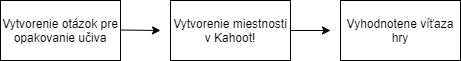
\includegraphics[scale=1.0]{diagram.pdf}
%\caption{Rozhodujúci argument.}
%\label{f:rozhod}
%\end{figure*}
\section{Iná časť} \label{ina}

Základným problémom je teda\ldots{} Najprv sa pozrieme na nejaké vysvetlenie (časť~\ref{ina:nejake}), a potom na ešte nejaké (časť~\ref{ina:nejake}).\footnote{Niekedy môžete potrebovať aj poznámku pod čiarou.}

Môže sa zdať, že problém vlastne nejestvuje\cite{Coplien:MPD}, ale bolo dokázané, že to tak nie je~\cite{Czarnecki:Staged, Czarnecki:Progress}. Napriek tomu, aj dnes na webe narazíme na všelijaké pochybné názory\cite{PLP-Framework}. Dôležité veci možno \emph{zdôrazniť kurzívou}.


\subsection{Nejaké vysvetlenie} \label{ina:nejake}

Niekedy treba uviesť zoznam:

\begin{itemize}
\item jedna vec
\item druhá vec
	\begin{itemize}
	\item x
	\item y
	\end{itemize}
\end{itemize}

Ten istý zoznam, len číslovaný:

\begin{enumerate}
\item jedna vec
\item druhá vec
	\begin{enumerate}
	\item x
	\item y
	\end{enumerate}
\end{enumerate}


\subsection{Ešte nejaké vysvetlenie} \label{ina:este}

\paragraph{Veľmi dôležitá poznámka.}
Niekedy je potrebné nadpisom označiť odsek. Text pokračuje hneď za nadpisom.



\section{Dôležitá časť} \label{dolezita}




\section{Ešte dôležitejšia časť} \label{dolezitejsia}




\section{Záver} \label{zaver} % prípadne iný variant názvu



%\acknowledgement{Ak niekomu chcete poďakovať\ldots}


% týmto sa generuje zoznam literatúry z obsahu súboru literatura.bib podľa toho, na čo sa v článku odkazujete
\bibliography{literatura}
\bibliographystyle{plain} % prípadne alpha, abbrv alebo hociktorý iný
<<<<<<< HEAD
\end{document}
=======
\end{document}
>>>>>>> 298a0562592e45ba4da56c05b112c56b65884fd4
